% LTeX: language=de-DE
\chapter{Evaluation}
	Im Folgenden sollen die mechanische Integrität und Performance des Systems mit Respekt auf die in \cref{sec:constructive limitations} formulierten Rahmenbedingenungen diskutiert werden.
	Im Vorfeld wurden mehrere Testfahrten auf urbanem Untergrund und entlang verschiedener Steigungen durchgeführt.
	Insgesamt wurde die verbaute Batterie hierbei dreimal von \qty{42}{\volt} (voll geladen) herunter auf \qty{31}{\volt} (\qty{10}{\percent} Restkapazität) entladen.
	Zurückgelegte Distanz und mittlere, sowie maximale Geschwindigkeit wurden mittels Navigationssoftware und GPS gemessen.
	% Da aus Sicherheitsgründen einige Testläufe auf der Werkbank durchgeführt wurden und Messungen per GPS jedoch eine tatsächliche Bewegung im freien zwingend erforderlich machen, wurden zusätzlich Logginginformationen der ESC ausgelesen, um aus Umdrehungen pro Minute und Anzahl der Umdrehungen Werte zur Geschwindigkeit rechnerisch ermitteln zu können.\par\medskip
	%
	\begin{figure}[h]
		\centering
		\includesvg[width=.8\textwidth, inkscapelatex=false]{Footage/AwesomeBoard Transmission CAD/Drawings/Drivetrain inclined}
		\caption[Zeichnung des Gesamtaufbaus]{Zeichnung des Gesamtaufbaus montiert als Hinterachse.}
		\label{fig:drivetrain inclined}
	\end{figure}
	\Cref{fig:drivetrain inclined} zeigt eine Zeichnung des Gesamtaufbaus des Systems mit zwei Motoren, den Unterbaugruppen der Motorhalterungen, den Rollen und den Truck montiert an der Heckseite des Decks in geneigter Position.
	Zum Vergleich ist der reale Aufbau in \cref{fig:real world assembly} zu sehen.
	\begin{figure}[h]
		\centering
		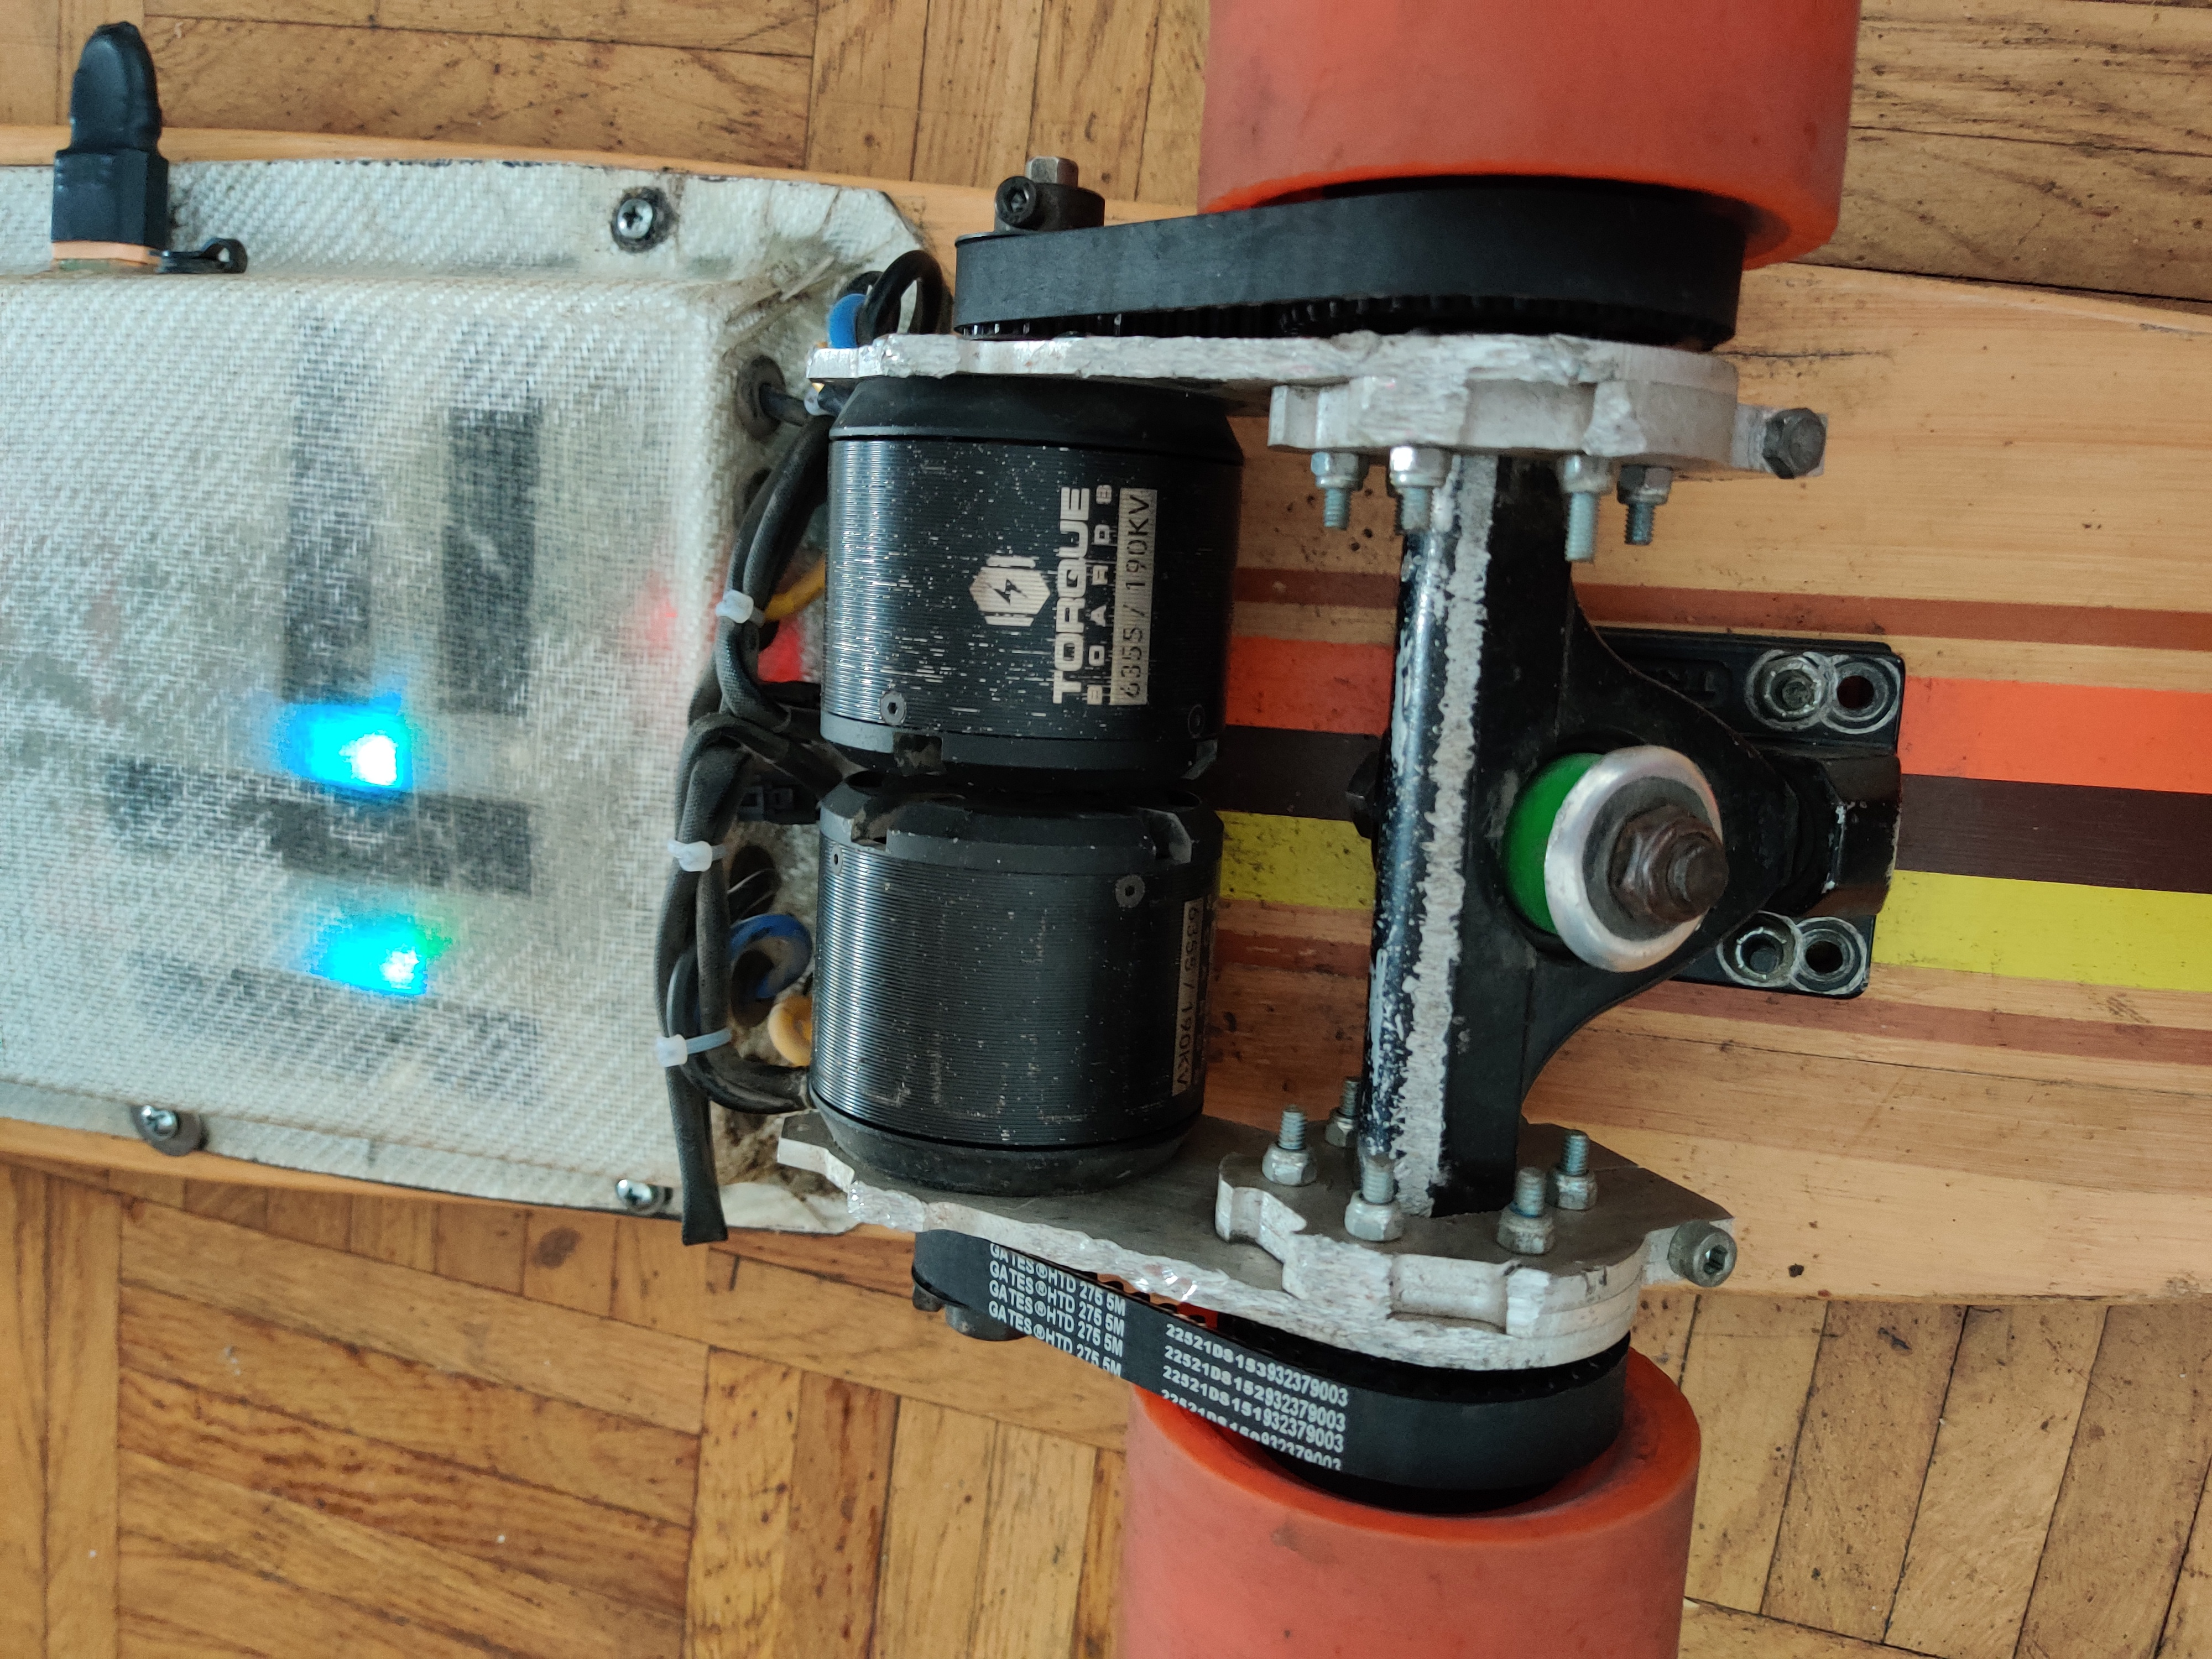
\includegraphics[angle=180, width=.5\textwidth]{Footage/Pictures/Drivetrain close up v2.jpg}
		\caption[Fertiger Aufbau des Antriebssystems]{Fertiger Aufbau des Antriebssystems nach etwa \qty{50}{\kilo\metre} Testfahrt durch urbanes Terrain.}
		\label{fig:real world assembly}
	\end{figure}

	\section{Performanz}
		Während mehrerer Testfahrten wurde das Drehmoment auf einer Strecke von etwa \qty{250}{\metre} entlang eines Hanges mit einer maximalen Steigung von \qty{7,5}{\percent} auf gepflastertem Untergrund getestet.
		Während das System aus dem Stand heraus nur schwer in der Lage ist zu beschleunigen, ist es ohne weiteres möglich mit moderater Anfangsgeschwindigkeit die Steigung zu überwinden.\par\medskip
		%
		Die Geschwindigkeitstests wurden entlang einer frisch asphaltierten, ebenen Strecke durchgeführt.
		Die theoretische Maximalgeschwindigkeit konnte hier aus Sicherheitsgründen nicht erreicht werden.
		Ab etwa \qty{20}{\kilo\metre\per\hour} wird das System zunehmend instabil und beginnt zu oszillieren.
		Via Software wurde nach \cref{eq:max speed by ERPM} die maximale Geschwindigkeit auf \qty{25}{\kilo\metre\per\hour} begrenzt, welche im Rahmen der durchgeführten Tests problemlos erreicht werden konnte.
		\begin{figure}[h]
			\centering
			\subcaptionbox{Ungenutzte Druckteile.\label{subfig:freshly printed pulleys}}[.49\textwidth][l]{
				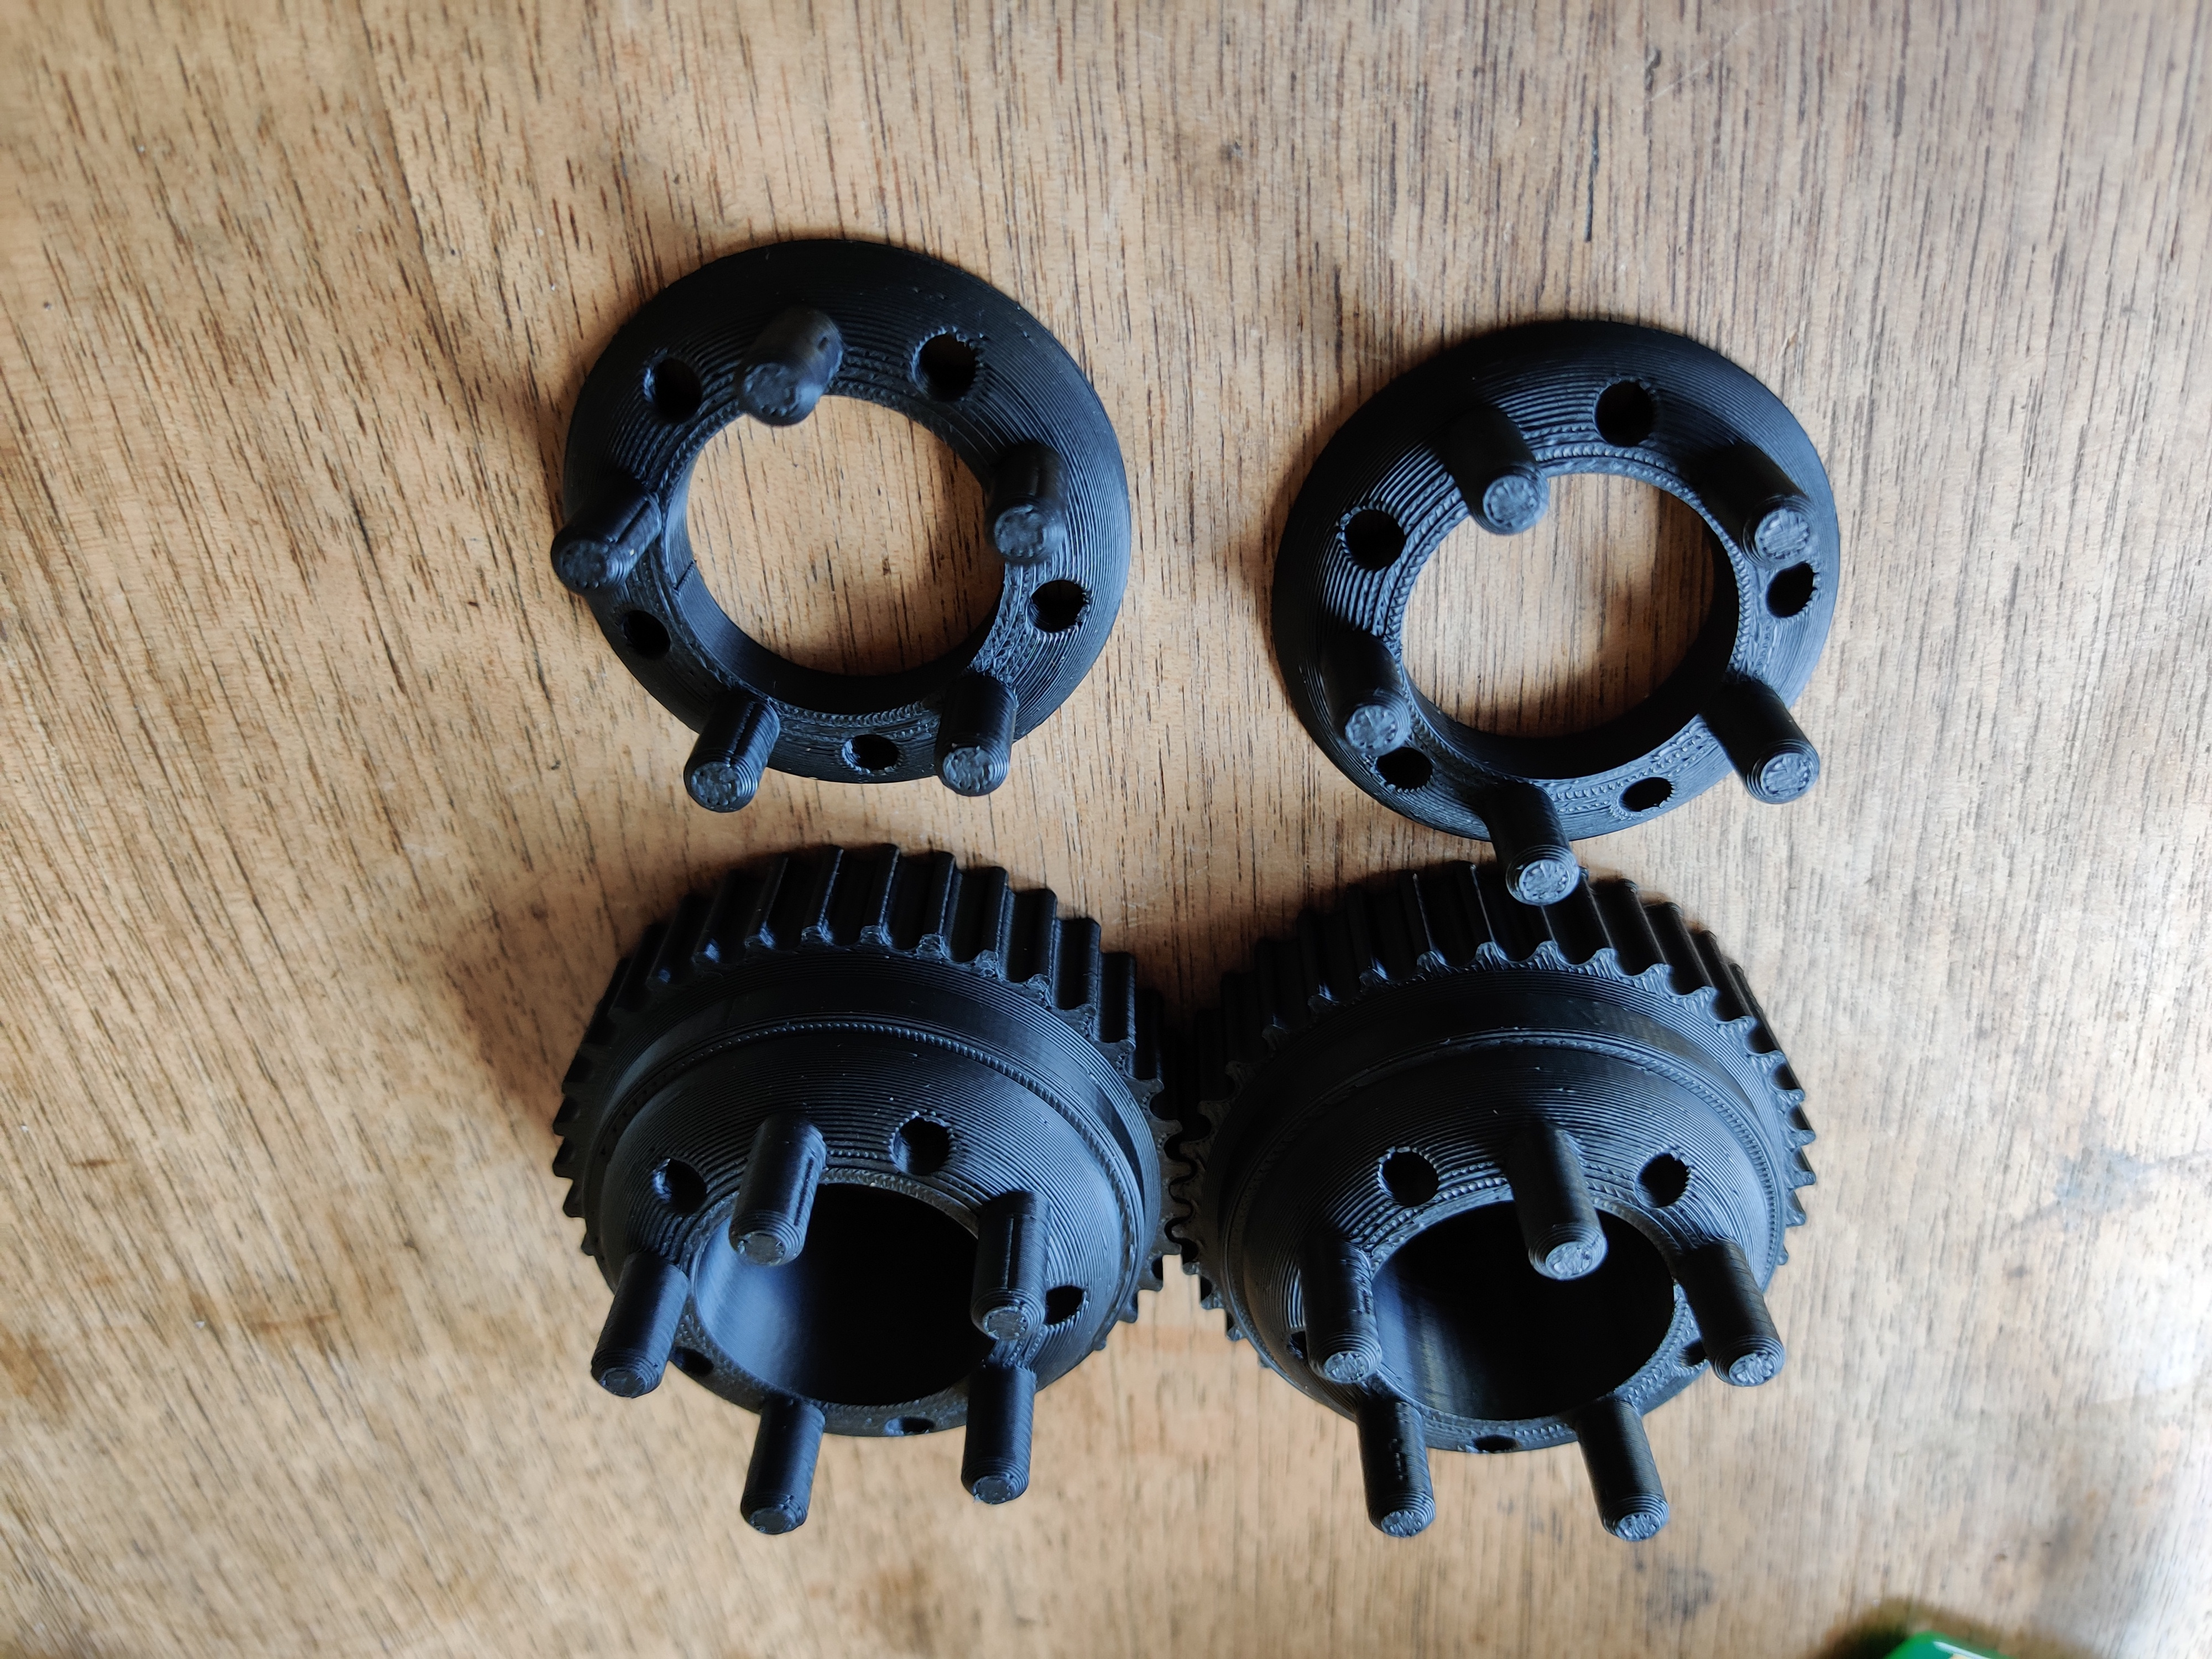
\includegraphics[angle=180, width=.49\textwidth]{Footage/Pictures/Wheel pulley v2.jpg}
			}
			\subcaptionbox{Zustand der Druckteile nach einigen Testfahrten.\label{subfig:printed pulleys after test driving}}[.49\textwidth][r]{
				\includegraphics[width=.49\textwidth]{Footage/Pictures/Wheel pulley v1.jpg}
			}
			\caption[Vergleich der gedruckten Zahn- und Konterscheiben vor und nach mehreren Testfahrten]{(a) Die finale und zum Zeitpunkt des Verfassens dieses Dokumentes noch verbaute Version. (b) Der Zustand des ersten funktionalen Prototypes nach etwa \qty{100}{\kilo\metre} Testfahrt. Neben zu erwartender Verschmutzung sei insbesondere auf das Fehlen der Führungsstifte zu achten. Das Zahnprofil und die Komponenten als ganze weisen darüber hinaus jedoch keinerlei Anzeichen von Materialversagen auf.}
			\label{fig:comparison printed parts used unused}
		\end{figure}